\chapter{\label{II_2}Description et indexation automatique} 

%à rajouter pour faire la transition : %L'apport de l'IA (Vers la classification sémantique) : La détection brute des coupures ne suffit plus ; l'enjeu actuel est la Shot semantics (décrire le contenu d'un plan et sa typologie) (Arnold  Tilton, 2019).

La description automatique d’images peut être centrée sur de nombreux éléments au sein d'une \gls{sequence} de film : dialogues, ambiance sonore, visages, objets, spatialité des éléments, actions, émotions... Toutefois, la définition d’un processus au sein d’un logiciel de gestion des collections impose un cadrage défini des fonctionnalités. Le corpus patrimonial retenu pour notre étude, constitué de \gls{rush} muets des premiers temps, exclue d’emblée l’analyse automatique de caractéristiques sonores. L’analyse automatique se concentre donc exclusivement sur les caractéristiques visuelles de l’image. Deux approches coexistent alors, celle de l’identification des éléments dans l’image de manière précise, ou celle d’éventuellement générer des résumés automatiques sur ces séquences, à une échelle plus globale. Or, la seconde approche, fondée sur des grands modèles de langage, implique des architectures génératives couteuses et lourdes. Nous choisissons ainsi d’adopter la première, afin de garantir une indexation fiable et stable, plus légère, à travers la détection et l’identification d’objets sur les \gls{imgcle}préalablement extraites. Cette tâche peut être réalisée par des architectures de réseaux de neurones relativement légers, pouvant extraire des concepts directement indexables au sein du logiciel.  




\section{\label{II_2_A}Outils utilisés}

Si pour la tâche de segmentation automatique, nous avons écarté les architectures de modèles fondés sur des réseaux de neurones, la reconnaissance d'objets dans l'image suppose une prédiction fondée sur un apprentissage machine profond des réseaux de neurones. En effet, la plupart des outils de reconnaissance d'objets dans l'image sont fondés sur des modèles de réseaux de neurones convolutifs (CNN) dont nous avons exposé le fonctionnement dans la section précédente. Dans le domaine du patrimoine, dont le logiciel de Skinsoft gère les données des institutions, se pose la question d'une infrastructure adaptée qui permet d'assurer la sécurité des données produites. Les solutions commerciales d'analyse automatique sont pour la plupart fondées sur un Cloud externe qui implique le déplacement des données. Ces solutions sont inadaptées au contexte d'analyse de données patrimoniales en raison de propriété intellectuelle et de sécurité. Ainsi, le principe retenu afin de guider notre choix d'outil est celui d'"amener l'algorithme aux données [Traduction personnelle]" \footnote{\textit{"bring algorithms to the data"}}, via un développement local interne des modèles d'analyse \footcite{noord2021}. Afin de répondre à cette contrainte, notre choix s'est trouné vers des modèles en libre accès. Nous détaillerons dans cette section l’utilisation de l’architecture \gls{yolo}, une série d’algorithmes dédiés à la détection d’objets visuels dans les images et les flux vidéo, et fondé sur les réseaux neuronaux convolutifs, développé par Joseph Redmond en 2015, puis repris par Ultralytics en 2020 \footcite{talbi2025}. 
C’est l’un des outils de détection d’objets les plus documentés, y compris dans le domaine des sciences humaines et du patrimoine. Fondé sur la \gls{Vision par ordinateur} et entraîné grâce à des méthodes d'\gls{Apprentissage profond}, \gls{yolo} est en accès libre, et permet notamment la détection d'objets et la classification d'images, permettant ainsi de poser les bases d’une indexation \footcite{jocher2022}. Le modèle extrait dans un premier temps les caractéristiques visuelles de l'image qui lui est donnée, les agrège, afin de finalement proposer une détection d'objets \footcite{norindr2023}. Les versions récentes du modèle telles que YoLo12 ne sont désormais plus seulement basées sur des \gls{cnn} mais sur des mécanismes d'auto-attention, similaires à ceux des \gls{Transformers} dont nous avions évoqué l'architecture \footcite{2025b}. Toutefois, comme nous l'avions évoqué, cette architecture demande une consommation de mémoire élevée et une puissance de calcul lourde \footcite{2025b}. Ultralytics, créateur du modèle, recommande des versions moins avancées pour une mise en application rapide, telles que la version Yolov8, uniquement fondée sur un réseau de neurones convolutif \footcite{2023c}. Yolov8 propose une version optimisée de cette architecture en trois temps : extraction, aggrégation, et détection \footcite{yaseen2024}. Le modèle se caractérise par sa capacité à analyser l'image en une seule fois, contrairement à d'autres modèles dont les résultats impliquent plusieurs analyses de certaines parties de l'image \footcite{redmon2016}.  
Si la détection d’objets prévue par \gls{yolo} peut être appliqué à des flux vidéo, nous souhaitons l'intégrer comme composant complémentaire au processus de segmentation précédemment décrit. De fait, il être pertinent de réutiliser l'image clé fixe, produite et sauvegardée par l'outil pyscenedetect, associée à chaque séquence, afin de la faire analyser par le modèle. Ceci permettrait de réduire le temps de calcul du processus et d'améliorer l'efficacité des prédictions, puisque le modèle reçoit un minimum d’informations.  
Ainsi, l’application du modèle \gls{yolo} s’impose comme la suite logique du pipeline de segmentation détaillé précédemment, afin d’indexer les segments produits, via l’utilisation des \gls{imgcle}. Si le premier processus de segmentation produit des données temporelles associées à chaque séquence sous la forme de time codes, \gls{yolo} produit des données sémantiques sur ces mêmes séquences. À l'issue de l'analyse d'une \gls{imgcle}, le modèle \gls{yolo} est capable de produire trois types de données : des étiquettes sur les objets identifiés, un score de confiance qui indique l'indice de certitude concernant la prédiction, des coordonnées spatiales de localisation de l'objet détecté dans l'image \footcite{redmon2016}. Les étiquettes produites sur les objets identifiés, permettant de décrire les caractéristiques de l’image, pourront être indexées comme des mots-clés au sein du logiciel de gestion des collections. Le processus de détection d'objets prévu par \gls{yolo} à partir de l'image clé peut être schématisé ainsi : 

\begin{figure}[H] 
	
	\centering 
	
	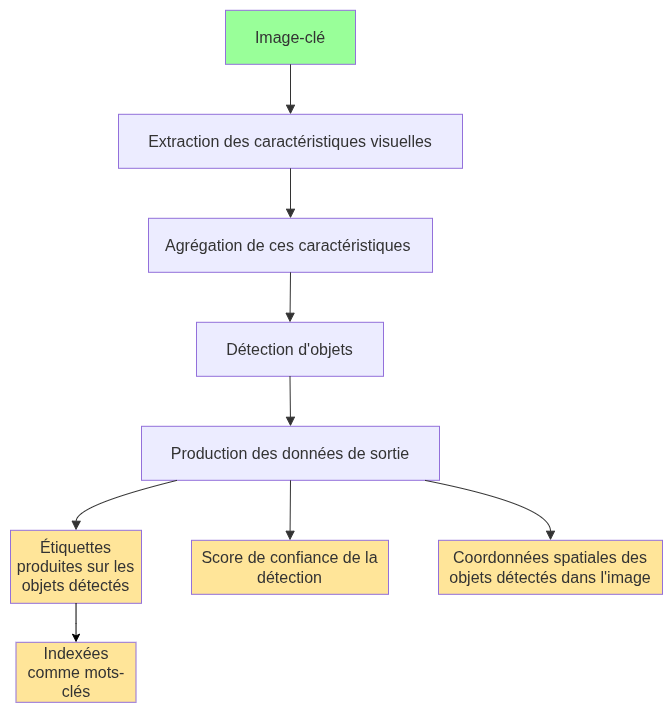
\includegraphics[width=0.7\textwidth]{images/yolo.png} 
	
	\caption{Processus de détection d'objets de \gls{yolo}} 
	
	\label{fig:yolo} 
	
\end{figure}

Les mots-clés produits à partir des étiquettes sont ensuite associés aux time-codes de chaque séquence détectée. Ainsi, chaque séquence contiendrait les données suivantes : des time codes qui l'identifient comme extrait, des étiquettes/mots-clés sur les objets qu'elle contient, et des données qui permettraient aux utilisateurs de vérifier la prédiction et de la valider. Le score de confiance produit par le modèle, permet en effet d'indiquer à l'utilisateur la certitude de l'étiquette associée à tel objet détecté. De même, les coordonnées spatiales de l’étiquette produite permettent à l’utilisateur de vérifier dans l'image si l'étiquette produite est associée au bon objet.  
\section{\label{II_2_B}Entraînement}

L'analyse automatique du contenu des images repose donc sur les architectures des \gls{cnn}, fondées sur des méthodes d'\gls{Apprentissage profond}, dont YOLO est un exemple concret. Toutefois, les algorithmes fondés sur l'\gls{Apprentissage profond} subissent généralement un entraînement supplémentaire afin d'analyse adéquatement le contenu des images en fonction d'un contexte donné. Deux approches méthologiques d'entraînement peuvent être appliquées, l'\gls{appsup} et l'\gls{appnonsup}. L'\gls{appsup} est fondé sur l'utilisation de données annotées pour l'amélioration des prédictions du modèle d'analyse d'image, tandis que l'\gls{appnonsup} exécute des tâches d'analyse et de classification à partir de données brutes, non annotées \footcite{delua2024}. Toutefois, l'\gls{appnonsup} ne permet pas d'adapter suffisamment le modèle de détection d'objets au corpus d'images spécifique étudié. En effet, si Yolov8 a toutefois fait l'objet d'un pré-entraînement en amont de sa mise à disposition, sur le jeu de données COCO, ce dernier, composé de 200 000 images annotées, reste généraliste et adapté à la détection d'objets communs et contemporain\footcite{2023b}. Or, l'efficacité des modèles basés sur l'\gls{Apprentissage profond} sur un corpus spécifique dépend fondamentalement de nature et de la qualité de leur données d'entraînement. 
Au sein des sous sections suivantes, nous prendrons comme exemple d’application le projet des archives britanniques en ligne, qui propose une chaine de traitement pour la détection d’objet basée sur l'\gls{Apprentissage profond} et la supervision humaine \footcite{kasturi2024}. Le projet, à travers la mise en place d'une supervision au sein du processus d'analyse par le modèle, propose de mettre en application le concept de \gls{hil} \footcite{kasturi2024}.
Le corpus étudié, caractérisé par l'ancienneté de ses images en fait un corpus d’images spécifique sur lequel l’algorithme doit subir un entraînement supplémentaire, supervisé. Afin d'adapter le modèle à notre corpus et ainsi d'en améliorer l'efficacité, une phase de pré traitement est nécessaire sur les données du corpus, au cours de laquelle des images sont sélectionnées afin d’être annotées pour être pré-testées par le modèle \footcite{kasturi2024}. La supervision humaine est déterminante dans ce processus, particulièrement dans le cas d’analyse de corpus inédits sur lesquels l’algorithme reste à entraîner \footcite{kasturi2024}. 
Les british online archives implémentent l'adaptation du modèle par la pré selection d'un nombre d'images définis, annotées manuellement à l'aide de la plateforme \gls{labels} \footcite{kasturi2024}. \gls{labels} est une plateforme open source déployable localement, qui permet ainsi de respecter la protection des données analysées \footcite{zotero-item-783}.
Afin d'éviter l'annotation manuelle de l'ensemble des \gls{imgcle} issues du processus de segmentation, il peut être envisagé d'exécuter au préalable \gls{yolo} depuis \gls{labels} sur l'ensemble des \gls{imgcle} du corpus afin de générer une base de prédictions \footcite{development2025}. Les détections brutes générées peuvent ensuite être importées au sein de la plateforme comme une couche d'annotation préalable à partir de laquelle affiner le modèle. Au sein de \gls{labels}, les prédictions s'affichent sous la forme de \textit{bounding boxes}, c'est-à-dire de boîtes englobantes autour des objets detectés dans l'image, avec le score de confiance qui y est associé \footcite{kasturi2024}. Le paramètre [choices] permet au modèle de proposer une classification sur les objets détectés, c'est-à-dire un mot clé \footcite{zotero-item-785}. Afin de focaliser la supervision du modèle sur les éléments les plus pertinents, il peut être décidé de ré annoter les images dont la détection est jugée incertaine par le modèle via un score de confiance en dessous du seuil minimal attendu \footcite{development2025}. Les archives brittaniques préconisent également la uppression des boites englobantes redondantes afin de sélectionner celles qui sont les plus pertinentes pour la supervision \footcite{kasturi2024}. Dans \gls{labels}, les utilisateurs (une équipe technique dans le cas de Skinsoft) examinent les prédictions ainsi générées sur les images, rectifient si besoin la définition des "boites" et la classification associée \footcite{kasturi2024}. Les données ainsi corrigées sont exportées au format \gls{yolo} depuis \gls{labels}, puis réinjectées dans la chaîne de réentraînement du modèle afin d'améliorer les performances en accord avec le corpus \footcite{kasturi2024}.
Cette méthode s'appuie sur le transfert d’apprentissage (transfert learning), qui consiste à \textit{fine tuner} un modèle existant, c’est-à-dire de l’affiner, afin de l'adapter au corpus analysé \footcite{bhargav2019}. À défaut de réentraîner le modèle dans sa globalité, les prédictions réalisées à partir du jeu de données d'entraînement COCO sont conservées puis spécialisées sur un corpus donné \footcite{bhargav2019}. L'affinage du modèle via la rectification et l'annotation des données, constitue une étape de prétraitement, en amont de l’analyse des données, afin d'améliorer l'efficacité de la détection d’objets \footcite{kasturi2024}.
Cette étape de pré-traitement, avant le processus d'analyse, implique la définition des types de mots clés souhaités, pour l'indexation des séquences. En effet, les étiquettes associées aux objets au sein des images correspondent aux mots-clés qui seront prédits par le modèle lors de l’analyse. Dans le cadre du corpus étudié, il est pertinent d’extraire les mots-clés déjà indexés sur les \gls{sequence} au sein du logiciel. Ces mots-clés varient selon le contenu de l’image et peuvent, par exemple, être les suivants : affiche, foule, policier, gendarme, drapeau, etc. Ces mots-clés, tout comme le jeu de données COCO, sont assez génériques. De fait, le pré traitement est avant tout utile pour l’entraînement du modèle à pouvoir détecter des objets au sein d’images dont la qualité est compromise.   
\section{\label{II_2_C}Processus de validation technique}

%Poursuite de l'application du concept HIL 

Afin de gérer les essais-erreurs de l'affinage du modèle sur les données spécifiques du corpus, il est pertinent de mettre en place un processus de validation technique du traitement. Ce processus permettrait d'une part de valider les résultats du modèle, et d’autre part, d'assurer la concordance entre les données produites par le modèle avec les données déjà existantes au sein du logiciel.

La validation des prédictions du modèle peut être effectuée au sein de la plateforme \gls{labels}. Les archives brittaniques proposent que le jeu de données test utilisé précédemment afin de corriger les prédictions, soit distinct d'un second jeu de données test, dédié à l'évaluation des performances du modèle, à différents niveaux de supervision humaine \footcite{kasturi2024}. Sur ce second jeu de données, sont notamment intégrées des métadonnées de supervision humaine. En effet, Kasturi explique l'introduction des notations "HIL-10 \%, HIL-15 \% et HIL-20 \%, qui signifient respectivement que les utilisateurs ont corrigé 10 \%, 15 \% et 20 \% des boîtes englobantes prédites peu performantes dans l’ensemble de données de test." \footcite{kasturi2024}. (traduction de :  HIL-10\%, HIL-15\%, and HIL-20\%, which signify that users have corrected 10\%, 15\%, and 20\% of poorly performing predicted bounding boxes in the test dataset, respectively). Les données corrigées manuellement remplacent ensuite certaines images au hasard dans le premier jeu de données d'apprentissage, contituant un nouveau jeu de données d'entraînement sur lequel le modèle s'affine \footcite{kasturi2024}. 
Le modèle ainsi affiné est finalement exécuté sur le second jeu de données, corrigé selon différents niveaux d'intervention humaine \footcite{kasturi2024}. Pour chaque niveau de supervision, sont analysés les "scores moyens d’Intersection over Union (mIOU) et de précision moyenne (mAP), ainsi que de la précision et du rappel" \footcite{kasturi2024}. 
Les résultats obtenus montrent que les performances du modèle s'améliorent considérablement à mesure que le pourcentage d'images corrigées manuellement augmente \footcite{kasturi2024}. En effet, l'enrichissement du jeu de données permet au modèle d'appréhender l'analyse des images de manière plus précise. L'auteur note toutefois la nécessité de poursuivre l'évaluation du modèle sur d'autres données afin de vérifier son adaptabilité et ses performances pour la détection d'autres types d'objets \footcite{kasturi2024}. En effet, le modèle devrait être ré entraîné constamment, à mesure qu'il soit exécuté sur de nouvelles données. (Active learning)


De plus, le processus de validation technique implique également la validation de l'indexation des données produites au sein du logiciel, en adéquation avec les règles métier en place. Au sein de l’espace de travail S-Movies dédié au corpus étudié, l'indexation des mots-clés est contrôlée par le thésaurus "keyword". Or, le modèle \gls{yolo} est nativement pré entraîné sur un jeu de données généraliste dont les étiquettes produites ne correspondront pas directement aux autorités indexées dans la base de données. Deux cas peuvent être gérés par l'utilisateur côté technique. D'une part, les mots-clés produits par le modèle peuvent déjà être indexés sous une forme contrôlée au sein du logiciel. Dans ce cas, il revient à l'utilisateur de vérifier que les mots-clés générés par le modèle concordent avec la forme indexée contrôlée au sein du logiciel. À terme, cette tâche de validation pourra être gérée par un LLM, un grand modèle de langage, déjà employé par Skinsoft pour un outil de recherche en langage naturel par exemple. Ce grand modèle de langage pourra être capable, à partir du thésaurus indexé dans le logiciel, de valider les formes contrôlées des mots-clés générés par \gls{yolo}. Pour cela, un mapping (tableau de corespondance) pourra être fourni au LLM entre les mots-clés que le modèle peut potentiellement générer, et leur forme contrôlée dans le thésaurus. Nous avons effectivement déjà élaboré un tel tableau au cours de notre stage dans le cadre de la mise en place de l'intelligence artificielle pour d'autres tâches, notamment la mise en place d'une recherche en langage naturel. Pour cette tâche tout à fait différente que celle que nous décrivons dans ce mémoire, nous avons effectué une table de correspondance entre les champs contrôlés pouvant être requêtés dans le logiciel et leur définition en langage naturel, préparant ainsi la gestion de synonymes et de termes employés par l'utilisateur potentiellement pour requêter ces champs. Sur le même principe, nous pourrions mettre en place une table de correspondance afin d'assurer la validation des données produites et d'assurer \textit{in fine} leur indexation au sein de l'application. Un calcul de similarité aide le LLM à repérer les termes simiaires et els rapprocher de leur forme contrôlée.
D'autre part, si les mots clés n'existent pas sous une forme contrôlée au sein du thésaurus et qu'aucune correspondance n'est détectée, un nouveau terme de thésaurus pourra être créé au sein du logiciel, avec l'accord de l'utilisateur.

%à ajouter : Named Entity Linking – NEL compare les entités trouvées avec les données normatives). L'algorithme ou le modèle mathématique effectue une classification multi-labels. Il se base sur des concepts statistiques tels que TF/IDF (Term Frequency/Inverted Document Frequency). \footcite{zotero-item-584}







La \gls{segtemp} ne se suffit pas à elle-même, mais nécessite une description du contenu des segments, afin d'en rétablir la qualité de \gls{sequence}, unité audiovisuelle à la fois syntaxique et sémiotique. L'approche retenue afin de décrire automatiquement le contenu de ces segments est celle de l'implémentation du modèle YOLOv8, dont le temps de calcul et de prédiction est réduit par son application aux \gls{imgcle} produites par la segmentation. L'efficacité du processus repose sur la supervision et la validation humaine, côté technique, des prédictions produites par le modèle, en accord avec les règles métier du logiciel. Toutefois, l'indexation définitive au sein du logiciel doit être validée par l'utilisateur métier via une interface dédiée, et au sein du modèle de données FRBR. 








%généralement, un algorithme de machine learning comprend trois étapes : data pre processing, data modelling, process optimisation. Dans le pre processing : humain requis pour transformer des données non structurées en données structurées et annotées \footcite{kasturi2024}

 










